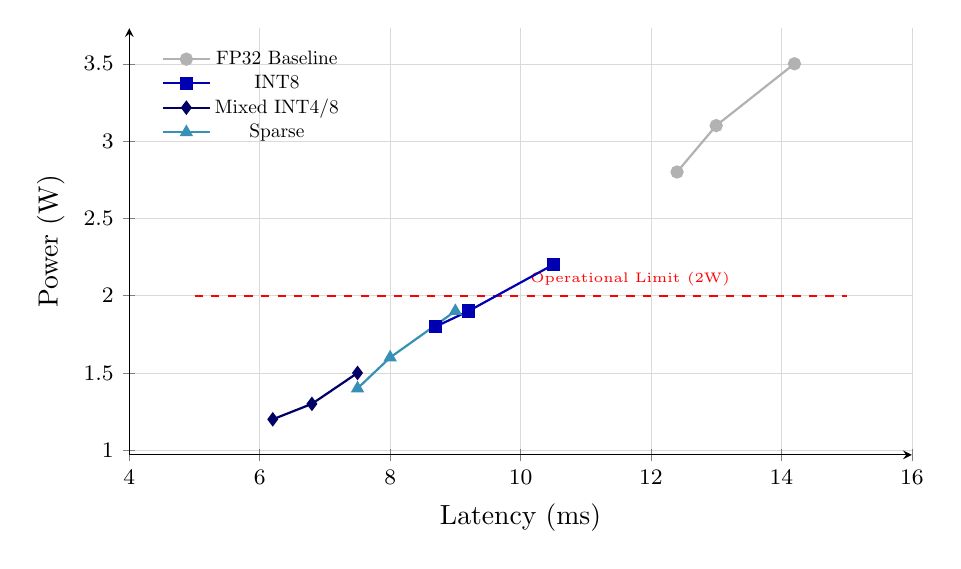
\begin{tikzpicture}
\begin{axis}[
    width=0.95\columnwidth,
    height=7cm,
    grid=both,
    grid style={line width=.1pt, draw=gray!10},
    major grid style={line width=.2pt, draw=gray!30},
    xlabel={Latency (ms)},
    ylabel={Power (W)},
    legend pos=north west,
    legend style={nodes={scale=0.7, transform shape}, draw=none, fill=none},
    axis lines=left,
    enlarge x limits=0.1,
    enlarge y limits=0.1,
    mark size=2pt,
    tick label style={font=\footnotesize}
]

% Límite Operativo Satelital
\addplot[red, dashed, thick, domain=5:15, forget plot] {2.0};
\node[red, anchor=south west] at (axis cs: 10, 2.0) {\tiny Operational Limit (2W)};

% FP32 Baseline
\addplot[color=gray!60, mark=*, thick] coordinates {
    (12.4, 2.8) (13.0, 3.1) (14.2, 3.5)
};
\addlegendentry{FP32 Baseline}

% INT8
\addplot[color=blue!70!black, mark=square*, thick] coordinates {
    (8.7, 1.8) (9.2, 1.9) (10.5, 2.2)
};
\addlegendentry{INT8}

% Mixed INT4/8
\addplot[color=blue!40!black, mark=diamond*, thick] coordinates {
    (6.2, 1.2) (6.8, 1.3) (7.5, 1.5)
};
\addlegendentry{Mixed INT4/8}

% Sparse
\addplot[color=cyan!70!black, mark=triangle*, thick] coordinates {
    (7.5, 1.4) (8.0, 1.6) (9.0, 1.9)
};
\addlegendentry{Sparse}

\end{axis}
\end{tikzpicture}